Machine learning is an increasingly popular data analytics technique commonly used in areas not limited to particle physics. It is useful in situations where a large amount of data produced or observed involves analysis that require better efficiency and computation time compared to traditional statistical techniques. In high energy physics, the use of machine learning has had a significant impact, for example, in the discovery of the Higgs boson using Boosted Decision Trees \cite{chatrchyan2012observation, aad2012observation, chen2015higgs}. \\


%-------------------------------------------------------------------------%
\section{Machine learning}
Machine learning  (ML) is an umbrella term for algorithms that ``learn" patterns from given data to give predictions through a process called \text{training}. It should be noted that there is a lower limit to the size of a dataset. For instance, for the number of entries $n$ and the number of variables $p$, if $p>n$ then there is not enough information for the classifier to train effectively\footnote{There are methods using regularization, for example, lasso, to deal with this issue \cite{james2013introduction}}. The preferred size for data is $p \ll n$ so that there is an abundance of information on which the classifier can train. There are two general categories in ML; \textit{supervised learning} and \textit{unsupervised learning}. Supervised learning requires data with labeled outcomes to build an effective classifier for the analysis of raw data, the results of which are unlabelled. Unsupervised techniques, on the other hand, are used when the data do not have labeled outcomes making them purely data-driven methods, unlike supervised techniques. Supervised techniques are commonly used in collider physics analysis as the simulation process allows as much data required to be generated, thus freely managing the size of data with labeled outcomes, resulting in the desired balanced data. \\

Training a classifier is relatively simple, with many choices available that are user-friendly, extremely versatile and deliver high performance. The classifiers are built by minimizing the selected error, otherwise known as a loss-function. The common loss-functions are simple metrics such as the \textit{Mean Squared Error (MSE)}, 
\begin{equation}
    MSE = \frac{1}{n} \sum\limits_{i=1}^{n}(y_i-\hat{y}(x_i))^2
    \label{eq:MSE}
\end{equation}
or the \textit{Root MSE (RMSE)},
\begin{equation}
    RMSE = \sqrt{\frac{1}{n}\sum\limits_{i=1}^{n}(y_i-\hat{y}(x_i))^2}
    \label{eq:RMSE}
\end{equation}
which perform well in general \cite{james2013introduction}. The error term is obtained by subtracting the predicted fit $\hat{y}_i$ at the $i$th observation with input parameters $x_i$ to the `true' fit $y_i$ \cite{james2013introduction}. Another high-performance loss-function is the negative log-likelihood function otherwise known as \textit{Log-Loss}
\begin{equation}
    l(x) = -\sum\limits_{i=1}^{n} \ln P(y_i| z_i) = \sum\limits_{i=1}^{n} \Big(-y_i z_i + \ln(1+e^{z_i}) \Big)
    \label{eq:logloss}
\end{equation}
for some regressor $z_i=\Tilde{\beta}^T x_i$ for a given $i$th observation in each $x_i$. The log-loss function is derived from the logistic function $g(z_i)=1/(1+e^{-z_i})$ and conditional probability. For a binary class problem with values of $y_i\in\{0,1\}$ the conditional probability is given by
\begin{equation}
    P(y_i| z_i) = g(z_i)^{y_i}(1-g(z_i))^{1-y_i}
\end{equation}
thereby simplifying to the logistic function for the background ($y_i=0$) and the inverse of $g(z_i)$ for the signal ($y_i=1$) \cite{knetml}. After some preliminary tests, including the three metric in Equations (\ref{eq:MSE})-(\ref{eq:logloss}), we found that the three metrics produced good results with the log-loss consistently performing the best on the basis of the accuracy of test classifiers. \\

When training a classifier, one must take care of \textit{overtraining}, a relatively common mistake. Overtraining\footnote{This is synonymous with overfitting data points with a higher-order polynomial to a given two-dimensional data, with the predictive power suffering as a consequence of overfitting.} happens when the parameters of the model are too restrictive in the model's ability to be flexible. The flexibility relates to how a model performs under various data of a similar nature. In other words, by limiting the model to perform well under a single dataset when training, we are limiting our ability to perform well in its predictive power in cases such as raw data from experiments. Overtraining is a mistake easy to prevent, and techniques to improve the performance of a classifier easily assure that this problem does not occur. The methods used in this project are \text{cross-validation} and \textit{hyperparameter grid-search}. \\

\begin{itemize}
    \item \textbf{Cross-Validation (CV)} \par
    Cross-validations (CV) is the task of partitioning training data to create a smaller set of training and test data and building smaller classifiers to perform tests \cite{james2013introduction}. The most common CV technique is the \textit{k-fold CV}, where the training data is randomly sampled into $k$ different subsets. The $k-1$ subsets are set as training data to build the classifier on, and the remaining subset is used to validate the classifier. This procedure is repeated $k$ times, where each classifier is scored on its accuracy. The overall result typically involves taking the $k$-fold average scores.  There are no strict guidelines for what the best value of $k$ is, but most ML users prefer to stick to either 5 or 10 because of its simplicity and performance \cite{james2013introduction}. \\
    
    \item \textbf{Hyperparameter Grid-Search} \par
    When building a classifier, it is difficult to find the parameters that boost its efficiency while being mindful of overtraining. A grid search can be done to solve this dilemma. A grid search utilizes CV at its foundations to test the efficiency of the selected parameters. By using this feature, several parameters can be tested with the best performing parameters that are used to train the original training data. The down-side to this, though, is that it is computationally expensive and multiple tests may even require some consistency in outcomes before some criteria are narrowed. \\
\end{itemize}

Fine-tuning parameters while cross-validating is not the only effective method for developing efficient classifiers. A common technique known as \textit{feature engineering} can be used to modify existing variables so that the accuracy of the prediction may improve the classifiers. A basic feature engineering was done in this project. It involved the rearrangement of the four jet entries so that the maximum $p _T$ jet with a $b$-tag is considered to be the $b$-jet originating from the top decay, and the following jets are ordered with $p_T$ values regardless of whether there is a $b$-tag or not. \\

The most popular algorithms used by the scientific community (not limited to physics) are Neural Networks (NNs) and Decision Trees (DTs) which work extremely well when used in the correct setting. In many communities, NNs are favoured over DTs. Nonetheless, multiple preliminary tests using the \textit{automl} feature from the \textit{h2o} package \cite{h2o} have shown that the tree-based method known as \textit{Extreme Gradient Boosting (EGB/XGBoost)} is most suitable for building our classifiers. In the chosen framework, which is R \cite{R}, the package with this available function is called \textit{xgboost}, whether available as a standalone use \cite{xgboost} or an extension of the h2o package \cite{h2o}.\\

%-------------------------------------------------------------------------%
\section{Tree-based methods and Extreme Gradient Boosting}
\label{sec:method}
We can intuitively think of tree-based methods as an extension to cut-based analysis (Recall Section \ref{sec:cut}). Instead of discarding selections that do not meet certain criteria, these selections may be further explored by the algorithm provided such selections exist. These splits are made by minimizing the chosen loss-function as discussed in the preceding section, making it difficult to infer the physical consequences of these splits. A simple diagram is depicted in Figure \ref{fig:tree}, where we see the criteria $x>a$ as our `root node' (the beginning of the tree), $y>c$, $f(x,y)$ and $g(x,y)$ as `decision nodes' (points that perform a split), and `branches' connecting the `terminal nodes'/`leaves' that is our prediction for the event signature. The mathematical formalism of a regression tree is described by
\begin{equation}
    T(X) = \sum_{i=1}^m c_i I(X\in R_i)
    \label{eq:DT}
\end{equation}
where $R_i$ is the partition of the predictor space corresponding to a leaf for $i=1,...,m$ non-overlapping regions. For each partition, $I(X\in R_i)$ is an indicator function that outputs predictions as one or zero given an observation $x_j\subseteq X$; either it is the signal or the background \cite{james2013introduction}. The regression tree creates an output between 0 and 1 that is weighted with some constant $c_i$. Using Figure \ref{fig:tree} as an example with $f(x,y)>b$ and $g(x,y)>d$ to predict a signal, the tree is formed as \\
\begin{equation}
    \begin{split}
        T(X) & = c_1I(x>a\cap y>c \cap f(x,y)>b)  
             + c_2I(x>a\cap y>c \cap f(x,y)<b)  \\
            & + c_3I(x>a\cap y<c) + c_4I(x<a \cap g(x,y)>d) + c_5I(x<a \cap g(x,y)<d)
    \end{split}
    \label{eq:DT_ex}
\end{equation}



\begin{figure}[htbp]
    \centering
    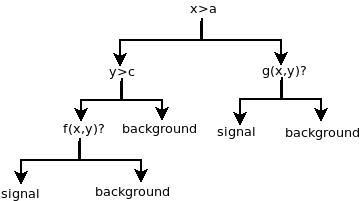
\includegraphics[width=10cm, height= 6cm]{DT.png}
    \caption{A diagram of a simple decision tree for a hypothetical signal selection following Figure \ref{fig:cut_flow} with an extra parameter $g(x,y)$ when $x<a$. The partition criteria in cut-based analysis were physically motivated and transparent, but the algorithm makes this process somewhat of a black-box, making direct physical interpretations challenging. The mathematical construction of this example tree is given by Equation (\ref{eq:DT_ex}).}
    \label{fig:tree}
\end{figure}

Most tree-based algorithms differ in the data sampling method and how the loss-function is minimized. In the case of EGB models, this is an extension to the \textit{Gradient Boosted Machine (GBM)} developed by Jerome Friedman \cite{friedman2001greedy}. \textit{Boosting} is an iterative algorithm in which an ensemble of weak models\footnote{A weak model consists of a small decision tree that is not an effective approximation to the data of interest.} are built sequentially, correcting its preceding model by re-weighting it with fitted errors from said model, leading to a final model that is highly representative of our data. Gradient boosting extends this idea with \textit{gradient descent}; an iterative algorithm that minimizes a differentiable loss-function, such as those in Equations (\ref{eq:MSE})-(\ref{eq:logloss}), to its local minima in its negative gradient direction specified by hyper-parameters \cite{gbmKaggle}. EGB/XGBoost adds to the features of regular GBMs with weighted quantile splittings and its ability to manage sparse\footnote{Since there are no missing entries in this project, the data is not sparse, or rather, it is `dense'.} data, incorporating parallel computing to achieve faster computation time compared to regular GBM algorithms \cite{chen2016xgboost}. We have been able to make the predictive power of our classifiers more accurate by considering certain hyper-parameters such as learning speed, depth and number of trees, and regularisation; a way to prevent overfitting by applying penalty terms, that can be tuned, to the loss-function  \cite{james2013introduction}. \\
%-------------------------------------------------------------------------%
\section{Metrics for model performance}
\label{sec:metrics}
%-------------------------------------------------------------------------%
\subsection{Confusion Matrix}
\label{sec:confMat}
The performance of a classifier can be summarized into a single table known as a confusion matrix. Displayed in Table \ref{tab:ConfMat}, a confusion matrix shows the distribution of correctly and incorrectly classified points predicted by the classifier. The correctly classified signal and background events are the True Positives (TP) and True Negatives (TN), respectively. Likewise, the incorrectly classified signal and background events are the False Negatives (FN) and False Positive (FP), respectively. The accuracy of the classifier is given by (TP+TN)/N and in a regression setting such as those in xgboost, a cut-off value between 0 and 1 varies this value. Choosing the ideal cut-off is important to maximize the Signal-to-Background Ratio (SBR)\footnote{The signal-to-background ratio is defined as the proportion of signal over the proportion of background events. In our analysis, we look to the cross-section and luminosity normalized TP and FP rates for signal and background respectively.} while maintaining high accuracy. \\

% Confusion matrix template
\begin{table}[htbp]
    \centering 
    \begin{tabu}{c|[2pt]c|c|c|c}
        \multicolumn{2}{c}{}&\multicolumn{2}{c}{Predicted}&\\
        \tabucline[2pt]{3-5}
        \multicolumn{2}{c|[2pt]}{}
        &\multicolumn{1}{c|}{Background} &\multicolumn{1}{c|[2pt]}{Signal} &\multicolumn{1}{c|[2pt]}{Total}\\
        \tabucline[2pt]{2-5}
        \multirow{\items}{*}{\rotatebox{90}{Simulated}}
        &\multicolumn{1}{c|[2pt]}{Background} & \multicolumn{1}{c|}{TN} & \multicolumn{1}{c|[2pt]}{FP} & \multicolumn{1}{c|[2pt]}{TN$+$FP} \\
        \cline{2-5}
        \multicolumn{1}{c|[2pt]}{}& \multicolumn{1}{c|[2pt]}{Signal} & \multicolumn{1}{c|}{FN} & \multicolumn{1}{c|[2pt]}{TP} & \multicolumn{1}{c|[2pt]}{FN$+$TP} \\
        \tabucline[2pt]{2-5}
        \multicolumn{1}{c|[2pt]}{} & \multicolumn{1}{c|[2pt]}{Total} & \multicolumn{1}{c|}{TN$+$FN} & \multicolumn{1}{c|[2pt]}{FP$+$TP} & \multicolumn{1}{c|[2pt]}{N}\\
        \tabucline[2pt]{2-5}
    \end{tabu}
    \caption{A confusion matrix for truth (simulated) and predicted labels and its components. The diagonal components are the correctly classified background (TN) and signal (TP) events. The off-diagonal components are the mis-classified background (FP) and signal (FN) events. }
    \label{tab:ConfMat}
\end{table}

%-------------------------------------------------------------------------%
\subsection{Approximate Median Significance}
\label{sec:AMS}
The statistical techniques introduced in Section \ref{sec:freqStat} requires calculating pdfs and test statistics that we did not have access to in the duration of this project. Instead, we turn to an evaluation metric presented in the Higgs Challenge \cite{adam-bourdarios_learning_2014} known as the \textit{approximate median significance (AMS)}, given by
\begin{equation}
    \text{AMS} = \sqrt{2\Big((s+b+b_r)\ln\Big(1+\frac{s}{b+b_r}\Big)-s\Big)}
    \label{eq:AMS}
\end{equation}
where $s$ and $b$ are the \textit{luminosity-normalized}\footnote{This includes the cross-section of the process.} TP and FP rates, respectively, and $b_r$ is a constant regularization term set at 10 introduced to not allowing $b$ approach zero, helping to reduce the variance of the AMS. We can obtain $s$ and $b$, by calculating
\begin{equation}
    s(b) = N_{s(b)}\times \epsilon_{s(b)} 
    \label{eq:N}
\end{equation}
where $N_{s(b)} = \sigma \int L(t) dt = \sigma \times 137$ fb$^{-1}$ \cite{thomson2013modern} is the number of expected events, and $\epsilon_{s(b)}=\text{(TP+FN)}_s/\text{N}$ $ \big(\text{(TN+FP)}_b/\text{N}\big)$  is the efficiency of the classifier given a dataset of size N. In our case, the test set, 1/3 of the combined data of roughly two hundred thousand events, was used to evaluate the AMS. The signal and background values when calculating the SBR we wish to maximize will refer to the value obtained via Equation (\ref{eq:N}) henceforth. \\

%The Gaussian significance discovery, discussed briefly in Section \ref{sec:freqStat}, with an estimated standard deviation\footnote{The standard deviation is actually given by $(n-\mu_b)/\sqrt{\mu_b}$ as the Poisson fluctuation of the background has a standard deviation of $\sqrt{\mu_b}$. Here, $n$ is the number of events and $\mu_b$ is the mean of the background. These numbers are replaced with their empirical counterparts: $s+b$ and $b$ respectively.} of $s/\sqrt{b}$ only hold when $s \ll b$ and $b\gg1$. This is not true in practice, therefore we turn to an approximate measure such as the AMS. 
%This measure is a derivation of the significance Z given by Equation (\ref{eq:Z})
%\begin{equation}
%    \text{Z} = \sqrt{2\Big( n\ln\Big(\frac{n}{\mu_b}\Big)-n+\mu_b\Big)}
%    \label{eq:Z}
%\end{equation}
%where $n$ is the number of events and $\mu_b$ is the mean of the background, requiring that $n>\mu_b$. The values $n$ and $\mu_b$ are replaced by $s+b$ and $b$ in Equation (\ref{eq:AMS}), respectively. Traditionally, the Z significane at $Z=5$ corresponds to a $p$-value of less than $2.9\times10^{-7}$, sufficient to claim a discovery \cite{adam-bourdarios_learning_2014}. However, the regularization term $b_r$ is equal to zero in this setting, thus differing this significance of values given by either equations. \\
%-------------------------------------------------------------------------%
\subsection{Feature Importance}
\label{sec:importance}

The simple tree diagram in Figure \ref{fig:tree} is not a practical tool to observe the structure and performance of the large number of trees created by algorithms such as xgboost. We then turn to \textit{feature importance} to quantitatively evaluate the performance of our classifiers with the variables used \cite{james2013introduction}. \\

XGBoost calculates feature importance in various metrics, one of which is the \textit{Gain} \cite{xgboost}. The `Gain' gives the contribution of each variable to the classifier as a fraction of the total gain from said variable upon splits. The gain of each split is defined as
\begin{equation}
    Gain = \frac{1}{2}\Bigg[ S_L + S_R + S_O \Bigg] -\gamma
    \label{eq:Gain}
\end{equation}
for scores on the new left(right) leaf $S_L$ ($S_R$) and the original leaf $S_O$. The penalty term $gamma$ regulates whether a split is created from a leaf i.e. if Equation (\ref{eq:Gain}) is negative, the leaf is not split \cite{xgboost_documentation}. 